\chapter{Background }
This chapter covers technologies which are relevant to the thesis. It starts with the overview of similar monitoring tools for cluster based applications and follows by short overview of tools for debugging of large scale applications. Later different approaches to applications profiling are described. 
In the next several sections the technologies which have been consider or are used in the thesis in the current moment are introduced. It covers libraries for bytecode manipulation, communication, logging and Java relevant libraries such as JNI and JVMTI. Docker is briefly described at the end of this chapter as it is used as the main distributed package for the whole platform.

\section{Cluster Monitoring Tools}
The most significant platforms to this thesis are Google Dapper and Zipkin, where Zipkin is based on the previous. Both serves the same core purpose which is to monitor large-scale Java based distributed applications. This thesis is based mainly on Google Dapper but also uses helpful Zipkin modules such as the user interface. Since Zipkin is developed according to Google Dapper design, these two platforms shares very similar concepts. The most important concept is a Span and it is explained in more details in the  following section. For now, we can think of a span as time slots encapsulating several calls from one node to another with well-defined start and end of the communication. The following two sections describes the basics the both mentioned platform. Both Zipkin and Dapper shares very similar concepts wo we just point out the most import parts relevant to the thesis.
\subsection{Google Dapper}
Google Dapper is proprietary software which was mainly developed as a tool for monitoring large distributed applications since debugging and reasoning about applications running on multiple host at the same time, sometimes written in different programming languages is inherently complex. Google Dapper has 3 main pillars on which is built:
\begin{itemize}
	\item Low overhead
	It was assumed that such a tool should share the same life-cycle as the monitored application itself thus low overhead was on of the main design goals as well. Google dapper 
	\item Application level transparency
	The developers and users of the application should not know about the monitoring tool and are not supposed to change the way how they interact with the system. It can be assumed from the paper that achieving application level transparency at Google was easier than it could be in more diverse environments since all the code produced in the Google shares the same libraries and control flow.
	\item Scalability
	Such a system should perform well on large scale data.
\end{itemize}	
Google Dapper collects so called distributed traces. The origin of the distributed trace is the communication/task initiator and the trace spans across the nodes in the cluster which took part as the computation/communication.
	
There were two proposals for obtaining this information - using the black-box and annotation-based monitoring approaches. The first one assumes no additional knowledge about the application whereas the second can use of additional information via annotations. Dapper is mainly using black-box monitoring schema since most of the control flow and RPC subsystems are shared among Google.
	
In Dapper, distributed traces are captured in so called trace trees, where tree nodes are basic units of work referred to as spans. Span is related to other spans via dependency edges. These edges represents relationship between parent span and children of this span. Usually the edges represents some kind of RPC calls or similar kind of communication.

Each span its own id so it can be uniquely identified. In order to reconstruct the whole trace tree, we need to be able to identify the starting Span. Spans without parent id are called root spans serves exactly that purpose. Span can also contain information from multiple hosts, usually from spans from direct neighborhood. Spans structure in Dapper platform is described in the figure \ref{fig:dapper_span}.
\begin{figure}
	\centering
		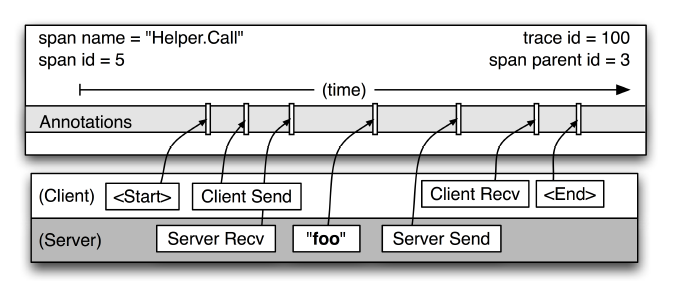
\includegraphics[scale=0.7]{dapper_span.png}
	\caption{Example of Span in Google Dapper. Picture taken from the Google Dapper paper}
	\label{fig:dapper_span}
\end{figure}

Dapper is able to achieve application-level transparency and follow distributed control paths thanks to instrumentation of a few common, mostly shared libraries among Google developers. 
\begin{itemize}
	\item Dapper attaches so called trace-context as thread-local variable to the thread when the thread handles any kind of control path. Trace context is small data structure containing mainly just reference to current and parent span via their ids.
	
	\item Dapper instruments the callback mechanism so when computation is deferred, the callbacks still carry around trace context of the creator and therefore also parent span ans current span id
	
	\item Most of the communication in Google is using single RPC framework with language bindings to different languages. This library was instrumented as well to achieve the desired transparency.
\end{itemize}

Even though Dapper is mainly following black-box monitoring scheme mentioned bellow, it still have small support for adding custom annotation to the code. This gives the developer of an application possibility to attach additional information to spans which are very application-specific.

The low-level overhead was also achieved by sampling the data. As is mentioned in the paper, the volume of data at Google is significant so only samples are taken at a time.

\subsection{Zipkin}
Zipkin is open-source distributed tracing system. It based on Google Dapper technical paper and manages both the collection and lookup of captured data.

Zipkin uses instrumentation and annotations for capturing the data. Some
information are captured automatically such as time when Span was created whereas some are optional and some even application-specific.

Zipkin architecture can bee seen on figure \ref{fig:zipkin_architecture}.
\begin{figure}
	\centering
	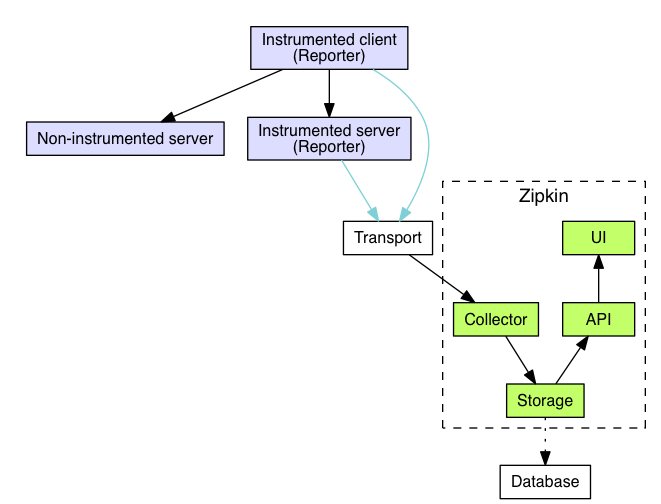
\includegraphics[scale=0.6]{zipkin_architecture.png}
	\caption{Zipkin architecture - http://zipkin.io/pages/architecture.html}
	\label{fig:zipkin_architecture}
\end{figure}
The instrumented application is responsible for creating valid traces. For that reason Zipkin has set of pre-instrumented libraries ready to be used which works well with whole Zipkin infrastructure. Spans are stored asynchronously in Zipkin to ensure lower overhead.

Once the span is created, it is sent to Zipkin, in more details, to Zipkin collector. In General, Zipkin consists of 4 components:
\begin{itemize}
	\item Zipkin Collector
	It is usually a daemon thread or process which stores, validates and indexes the data for future lockups.
	\item Storage
	Data in zipkin can be stored in a mulltiple ways, so this is a pluggable component. Data can be stored in for example in Cassandra, MySQL or can be send to Zipkin UI right away without storing it anywhere. The last option is good only for small amount of data.
	\item Zipkin Query Service
	This component act as a query daemon allowing us to query various informaion about span using simple JSON API.
	\item Web UI
	Basic, but very useful user interface. The user can see whole trace trees and all spans with dependencies between them.
\end{itemize}
 In the thesis the Zipkin UI is used as front end for developed the monitoring tool and it's format is described in more detail in  \hyperref[sec:zipkin_ui]{Zipkin UI} section of \hyperref[chap:design]{Design} chapter.
 
 The reason why Zipkin UI was selected as the primary user interface for this work is mainly it's simplicity and ease of use. Also it fulfills the visualization requirements of the thesis as well, since we need to see dependencies between spans and also whole trace tree as well. However the monitoring platform is not tightly-coupled with this user interface. We will see later how to create custom span savers which can store data in any format suitable for different visualization tools.
 

\section{Tools for Large-Scale Debugging}
Standard techniques and tools can be used for debugging distributed applications, however when using these tools we lack the information about dependencies between different nodes in the cluster. There are many tools under the category of large-scale debugging but we just point out basic ideas behind two different approaches - discovering scalling bugs and behaviour based debugging. 

\subsection{Discovering Scaling Bugs}
In distributed systems the scalability is very important. It is very important to know how our platform scales when it comes to significantly big data and what is the scalability trend we can expect. It can happen that on large data the platform can run significantly slower than expected when tested on smaller data. We call this issue as a scaling bug. Tools which can be used to help with these kind od bugs are for example Krishna and WuKong. Both of the mention tools are based on the same idea. They build a scaling trend based on data batches of smaller size. The observed scalling trend acts as a boundary. We observe the scalling bug when the scalling trend is violated. In the first tool, Wrishna, we can't tell which port of the program violated the scalling trend, however it is possible in the second tool, WuKong. In comparison to Krishna, Wukong doesn't build one scalling trend of the whole applications, but creates more smaller models, each per some control flow structure in desired programming language where the all these smaller models represent together the whole scalling trend. When we hit into scalling bug, WuKong can give us hints where the trend can be violated.

\subsection{Behavior-based Analysis}
The different category of tools used for debugging of large scale applications are based on behaviour analysis. The basic idea behind these tools is that the classes of equivalence are created from different program processes and different runs. Using this approach we lower down the number of data we need to inspect and the tools can help us to discover anomalies between different observed classes. For example, STAT - Stack Trace Analysis Tool, is a lightweight and scalable debugging tool used for identifying errors on massive high performance computing platforms. It gathers stack traces from all parallel executions, merges together stacktraces from different processes that have the same calling sequence and based on that creates equivalence classes which make it easier for debugging highly parallel applications. As the other example falling under the same category is AutomaDed. This tool creates several models from an execution and can compare them using clustering algorithm with (dis)-similarity metric to to discover anomalous behaviours. It also can point to specific code region which may be causing the anomaly.

\section{Profiling Tools}
Profiling is a form of dynamic code analysis used for analyzing for example how long each part of the system takes in the whole computation, where the computation spends the most time or the memory requirements of the whole program. Generally, we can group the profiling tools into two categories: sampling profilers and instrumentation profilers.

\begin{itemize}
	\item sampling profilers

Sampling profilers take statistical samples of an application at well-defined points such as method invocations. It usually have less overhead comparing to instrumentation profilers. The points were the application should take samples can be inserted at the compilation time by the compiler. Using these profilers we can collect how long the method run, who call it or for example the complete stacktrace. We however can't record any application specific information.
\item instrumentation profilers
This can be solved by instrumentation profilers. These profilers build on the instrumentation of the application's source code. They record the same kind of information as the sampling profilers but usually give us the ability to specify extra points in the code we are interested in and also to record application specific data.
\end{itemize}


However, we can look on profilers from different point of view and categorize them based on the level on which they operate and are able to record the information - system profilers and application specific profilers. 
At application specific profilers, we are the most interested in profilers targeted for JVM platform.
\begin{itemize}
	\item system profilers
	System profilers operate on OS-level. They are great at showing system code paths, but are not able to capture method calls done for example in Java application.
	\item JVM profilers
	These profilers show Java methods, but usually not system code paths.
\end{itemize}
The ideal solution for monitoring purposes would be to have information from both kind of profilers, however combining outputs of these profiler types is not straightforward. The profilers which are able to collect traces from both the profiler types are usually called mixed-mode profilers. JDK8u60 comes with the solution in a way of extra JVM argument \textit{-XX:+PreserveFramePointer} \cite{MixedModeProfilers}.  Operating system is usually using this field to point to most recent call of the stack frame and system profilers make uses of this field. In case of Java, compilers and virtual machines don't need to use this field since they are able to calculate the offset of the latest stack frame from the stack pointer. This leaves this register available for various kind of JVM optimalizations.

This option ensures that JVM abides the frame pointer register and will not use it as general purpose register and therefore we can get both system and JVM stack frames in a one call hierarchy. Using the JVM mixed-mode profilers we are able to collect information about:
\begin{itemize}
	\item page faults
	They allow us to see what leads to from of JVM resident memory.
	\item context switches
	Context switches are interesting to see code path leads to leaving the CPU.
	\item disk i/o requests
	Show code paths leading to IO operations such as blocking disk seek operation.
	\item TCP events
	Show code paths leading from high-level Java code to low-level system methods such as connect or accept, so we can reason about performance and good design of network communication in much more better detail.
	\item CPU cache misses
	Show code paths leading to cache misses. Using this information we can optimize the Java code to make better use of the existing cache hierarchy.
\end{itemize}

All the information bellow can be described on a special chart called Flame charts.
\subsubsection{Flame Charts}
Flame Chart is a concept by a developer Brendan Gregg. Flame graphs are aa visualization for samples stack traces, which allows the hot paths in the code to be identified quickly. The output of sampling of instrumentation profiler can be significantly big and therefore visualizing can help to reason about performance in more comfortable way. 

\begin{figure}
	\centering
	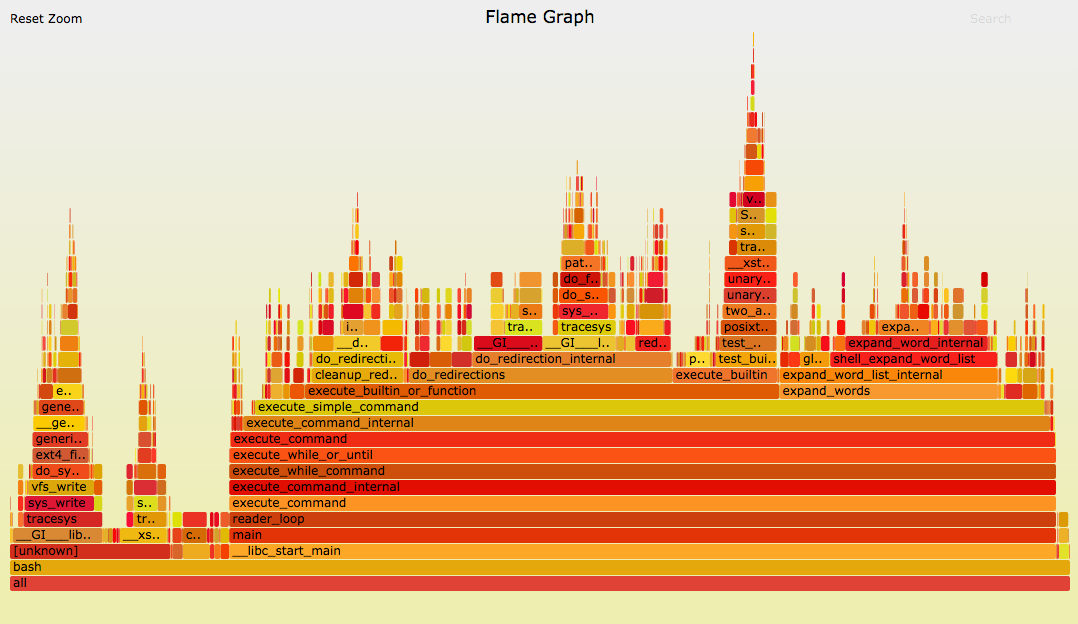
\includegraphics[scale=0.35]{flame_chart.png}
	\caption{Flame Graph example}
	\label{fig:flame_chart}
\end{figure}
The description:
\begin{itemize}
	\item Each box represents a function call in the stack
	\item The \textbf{y-axis} shows stack frame depth. The top function is the function which was at the moment of capturing this flame chart on the CPU. All functions underneath of it are its ancestors.
	\item The \textbf{x-axis} shows the population of traces. It doesn't represent passing of time. The function calls are usually sorted alphabetically.
	\item The width of each box represents the time the function was on CPU.
	\item The colors are not significant, they are just used to visually separate different function calls
\end{itemize}

Flame charts can be created in a few simple steps, but it depends on the type of profiler the user wants to use. 
\begin{enumerate}
	\item Capture stack traces
	For this step we can use profiler of our choice.
	\item Fold stacks
	We need to prepare the stacks so Flame graphs can be created out of them. For this, there are several scripts prepared for different profiler types.
	\item Generate the flame graph itself, again using the prepared script provided on the link above.
\end{enumerate}

Purpose of this really short section was just to introduce the idea of Flame charts since it's one of the future plans the thesis could be extended to support. For more information about the flame charts please visit the Brendan Gregg's blog.
\section{Bytecode Manipulation Libraries}
This thesis highly depends on the instrumentation for which the byte-code manipulation is a core feature. Since the work is written in Java, we are mainly interested in instrumentation and byte-code manipulation libraries based on Java. This section covers . The purpose of this section is to introduce 4 standard bytecode manipulation libraries - Javassist, ByteBuddy, CGlib and ASM - and give their comparison. Since it's a core feature of the whole platform and affect the performance and the usability of the whole platform, the library was thoroughly reviewed before selected. ByteBuddy was selected to be used in the thesis and the reasons why are mentioned bellow as well.

\subsection{ASM}
ASM is a low-level high-performance Java bytecode manipulation framework. It can be used to dynamically create new classes or redefined already existing classes. It works on the bytecode level so the user of this library is expected to understand the JVM bytecode in detail. ASM operates on event-driven model as it makes use of Visitor design pattern to walk through complex bytecode structures. ASM defines some default visitors such as \textit{FieldVisitor}, \textit{MethodVisitor} or \textit{ClassVisitor}. The ASM project can be a great fit for project requiring a full control over the bytecode creation or inspection since it's low-level nature.
\subsection{Javassist}
Javassist is well-known bytecode manipulation library built on top of ASM. It allows to Java programs to define new classes at runtime and also to modify a class files prior the JVM loads them. It works on higher level abstraction so the user of this library is not required to work with the low-level bytecode. The code to be injected to the existing bytecode is expressed as Java Strings which has the disadvantage that the code to be injected is not subject to code inspection in most of the current IDEs. The advantage of Javassist is that the injected code does not depend on the Javassist library at all. 
The strings representing the code are compiled on runtime by special javassist compiler which works well for most of the common programming structures but just to point out auto-boxing and generics are not supported by the compiler.
Javassist does not have support for the code injection itself. Therefore, it can be used for specifying the code which alters the original code but external tool needs to be used to inject the code.
\subsection{CGlib}
CGLib as another byte-code manupulation library built on top of ASM. The main concepts are build around `Enhancer` class which is used to create proxies by dynamically extending classes at runtime. The proxified class is then used to to intercept method calls and the result of previous methods or fields as we define. However cglib lacks comprehensive documentation making harder to even understand the basics from the users.

\subsection{Byte Buddy}
ByteBuddy is fairly new, light-weight and high-level bytecode manupulation library. The library depends only on visitor API of the ASM library which does not further have any other dependencies. It does not require from the user to understand format of java bytecode but despite this, it gives the users full flexibility to redefine the byte code according their specific needs. Also, classes created or instrumented by Byte Buddy does not depend on the Byte Buddy framework. Despite it's high-level approach, it still offers great performance and is used at frameworks such as Mockito or Hibernate. Byte Buddy can be used for both code generation and transformation of existing code.

\subsubsection{Code Generation}
Code generation is done by specifying from which class we want to create a subclass, in the most generic way we can create subclass from Object class. The newly created class can introduce new methods or intercept methods from it's super class. In order to intercept existing methods and change their behavior and return value, the method to be intercepted has to be identified using so-called ElementMatchers. These matchers allow us to identify methods using for example their names, number of arguments, return methods or associated annotations. The whole list of matchers and also examples how code can be generated is greatly described on the project Github page.

As mentioned earlier, the power behind Byte Buddy is also that it can be used to redefine classes at runtime. This is achieved several concepts, mainly Transformers, Interceptors and Advice API.
\subsubsection{Code Transformation}
In order to tell byte buddy when it needs to intercept a method or field, we need to identify the place in the code which triggers the interception. First,  the class containing method to be instrumented need to be located. It can be done by simply specifying the class name or using more complex structures. For example we can only consider all classes A extending class B whilst implementing interface C at the same type. 

The next step is to define the transformer class itself. Transformers are used to identify methods in the class which should be instrumented and they also specify what interceptor or advice should handle the instrumentation for the particular matched method. Such methods can be again identified using the ElementMatchers mentioned in the section above. In more detail, transformer interface has a method transfrom which has DynamicType.Builder as it's argument. This builder is used to create a single transformer wrapping all the previous ones for all classes in the code so the result of this builder can be thought of as a dispatcher of the instrumentation. Methods to be instrumented are specified on the builder instance using the ElementMatchers  as well as what interceptor or advice API will be used to handle the transformation.

As mentioned above there are 2 ways how to instrument a class in ByteBuddy.
\subsubsection{Interceptors}
Interceptor is a class defining the new or changed desired behavior for the method to be instrumented. 
We demonstrate how Byte Buddy uses interceptors on a small example. Let's assume we have original class Foo:
\begin{lstlisting}[language=Java]
class Foo {
	String bar() {
		return "bar"; 
	}
}
\end{lstlisting}
	
Le'ts also assume that our Interceptor is of type Qux. The interception of the class Foo using our interceptor looks like this in schematic code:

\begin{lstlisting}[language=Java]
class Foo {
	// Requires your interceptor class to be known
	static Qux $interceptor;
	String bar() {
		return $interceptor.intercept(); 
	}
	static {
		// Requires knowing the framework
		$interceptor = ByteBuddyFramework.defineField(Foo.class);
	}
}
\end{lstlisting}
		
We can therefore see that in case of interceptors, Byte Buddy does not inline the byte code to the \texttt{Foo} class but requires the interceptor class to be available on the machine where instrumentation takes place. Also the interceptor field needs to be initialized, which is in this case done in the static initializer. The initialization of interceptors is done using special helper class called \texttt{LoadedTypeInitializer}.

There are multiple ways how this behavior can be changed:
\begin{enumerate}
\item In Byte Buddy, initialization strategy can be modified according to the specific needs. We can define no-op strategy and read \texttt{LoadedTypeInitializer} right before the class is about to be instrumented.  Later we can perform the initialization our self using observed initializer or we can even serialize this initializer together with the \texttt{Qux} \texttt{Interceptor} class, send them to different JVM where the instrumentation should take place and manually initialize the the interceptor field.
\item Instead of referring to \texttt{Qux} as a instance, we can delegate to \texttt{Qux} as a class and call the interception logic via static methods. In this case the interceptor class still needs to ne known at runtime, but there is no need to perform the interceptor initialization.
\item Instead of using interceptors, advice api which inlines the code to the class itself may be used.
\end{enumerate}
\subsubsection{Advice API}
Advices are another approach how code can be instrumented in Byte Buddy. Compared to \texttt{Interceptor}s it is more limited, but on the other hand, in cases where it's possible to use it, the code is in-lined into the class's bytecode and therefore no other dependencies are required. It is also stated in Byte Buddy documentation that performance of Advice API is better compared to using interceptors.

However, instrumentation using Advice API is only allowed before or after the matched method which is achieved using the \texttt{Advice.onMethodEnter} and \texttt{Advice.onMethodExit} annotations.

\section{Communication Middleware}
This thesis consist of several parts which need be able to communicate. The communication is also complicated by the fact that the parts are written in different programming languages - Java and C++. In order to achieve communication in such an environment, following libraries has been inspected.
\subsection{Raw Sockets}
We are not referring to a library but to using raw sockets on their low-level API. Using raw sockets has several pros and cos. It give us a full flexibility and the highest possible performance since there isn't any additional layer between our application data and the socket itself. However, integrating different platforms and different languages can be time-consuming. Several frameworks have already been created to achieve this so the user does not need to know about the language or underlying platform.
\subsection{ZeroMQ}
ZeroMq is a communication library build on top of raw sockets. The core of the library is written in C++ however binding into different languages exist. The library is able transport messages inside a single process, between different processes on the same node, using TCP or also using multicast.

The library also supports to create typologies using one of many supported communication patterns like publisher-subscriber or request-reply.
\begin{itemize}
	\item Hiding the differences of underlying operating systems.
	\item Message framing - delivering whole messages instead of stream of bytes
	\item No need to worry about queuing messages. The internals take care of ensuring the messages are sent and received in correct order. The user can send the messages without knowing whether there are other messages in the queue or not.
	\item Language mappings to different languages.
	\item Ability to create a topologyy. For example, one socket can be connected to multiple endpoints.
	\item Automatic TCP re-connection
	\item Zero-copy
\end{itemize}
\subsubsection{Zero-copy in ZeroMQ}
The library also tries to apply concept called zero-copy if possible. When high-performance is expected from a system or network, copying of data is usually considered harmful and should be minimized as possible. The technique of avoiding copies of data is known as zero-copy.

Example of data copying is transferring data from memory to network interface or from user application to underlying kernel.  We can see that zero-copy can't be implemented at all layers because for example without copying the data from the kernel to network interface, we could not actually exchange any data. However, ZeroMQ can achieve zero-copy at least on the application message level so the users can create ZeroMQ messages from their data without any copying which is a big performance plus.
\subsection{NanoMsg}
NanoMsg [http://nanomsg.org/documentation-zeromq.html] is a socket library shadowing the differences in the underlying operation systems. It offers several communication patterns, is implemented on C and does not have any other dependencies. Generally, it offers very similar features to ZeroMQ since it's heavily based on it.

Unlike ZeroMQ, nanomsg matches the full POSIX compliance. The author of the library states, that since it's implemented in C, the number of memory allocations is drastically reduced compared to c++ when using C++ STL containers for example. Also compared to ZeroMQ, objects are not tightly bound to particular threads this it gives the user flexibility to create their custom threading models without big limitations. NanoMsg should also implement zero-copy technique at additional layers which again leads to performance benefits.

As in ZeroMQ, NanoMsq supports the following transport mechanisms:
\begin{itemize}
	\item \textbf{INPROC}
	Used for transporting messages withing a single process, for example between different threads. In-process address is arbitrary case-sensitive string starting with \texttt{inproc://}
	\item \textbf{IPC} - inter processes communication
	It enables several processes to communicate on the same node
	The implementation uses native IPC mechanism available on the target platform. On Unix-like systems, IPC addresses are just references to files where both absolute and relative path can be used. The application has to have rights to read and write from the IPC file in order to allow the communication.
	On Windows, the named pipes are used. The address can be arbitrary-case sensitive string containing any character but backslash. On both mentioned platforms, the address has to start with \texttt{ipc://} prefix.
	\item \textbf{TCP}
	TCP is used to transport messages in a reliable manner to a single recipient to in a reachable network. When connecting to a node, the address in format \texttt{tcp://interface:port} needs to used and when binding a node, address in format texttt{tcp://*:port} should be used.
\end{itemize}

NanoMsg can be used in via it's core C library, but also several language mappings for different languages exist.
\subsubsection{C++11 Mapping}
Nanomsgxx [https://github.com/achille-roussel/nanomsgxx] is a C++11 mapping for nanomsg library. It is a small layer build on top of core library making the API more C++11 like friendly. Especially, there is no need to tell when to release resources, since it's handled automatically in desctuctors. The \texttt{nnxx::message} abstraction over NanoMsg \texttt{nn::message} automatically manages buffers for zero-copy and also errors are reported using the exceptions which are sub-classes from \texttt{std::system\_error}

\subsubsection{Java Mapping}
Several Java bindings of nanomsg library exists, but just jnanomsg library [http://niwinz.github.io/jnanomsg/latest/] is described here. This language binding is build on top of JNA - Java Native Access library. It offers all the functionalities offered by the core library but also introduces non-blocking sockets exposed via a callback interface.
\section{Java Libraries}
This section describes some fundamental Java related libraries on technologies on which this thesis heavily depends. Firstly, Java Virtual Machine Tool Interface (JVMTI) is described followed by basic introduction to Java Native Interface. Important Java concepts and classes relevant to the thesis are described in the following few sections.
\subsection{JVMTI}
The JVM Tool Interface https://docs.oracle.com/javase/7/docs/platform/jvmti/jvmti.html is a interface used by development and monitoring tools for communication with JVM. It allows its user to monitor and control the execution running in Java virtual machine. An application communicating with the JVM using JVMTI is usually called agent. Agents are notified of the events happening inside JVM and can react upon them.

Agents run in the same process as the application itself this reducing the communication. Since JVMTI as interface written in C, agents can be written in C or C++. The agent has to be attached to the application via 

JVMTI supports 2 modes how agent can can be started, either in OnLoad phase or in Live phase. In OnLoad phase, client is started together with the application and agent location can be specified using 2 arguments:
\begin{itemize}
	\item \texttt{-agentlib:<agent-lib-name>=<options>} \newline
	In this case, the library name to load is specified and it is loaded using platform specific manner .
	\item \texttt{-agentpath:<path-to-agent>=<options>} \newline
	In this case, the path to a location of the library is specified and the library is loaded from there.
\end{itemize}

In the Live phase, the agent is dynamically attached to running application. This approach can be though as more flexible since we don't have to specify agent library to monitored application in advance, but it brings several limitation as well.

We don't aim to describe full JVMTI functionality here, please consider this just as brief introduction to the interface and inspect the documentation for more information. In the following sections we aim to very briefly describe the important parts of JVMTI relevant to the thesis.

\subsubsection{JVMTI Agent Initialization}
When client is started, the method \newline \texttt{Agent\_OnLoad(JavaVM *jvm, char *options, void *reserved)} is called. In this method we can do custom initialization for our agent.

Usually the initialization consist of several phases:
\begin{enumerate}
	\item Optionally, parse arguments passed to JVMTI agent.
	\item Initialize JVMTI environment in order to be able to communicate with the observed application. JVMTI does not handle threads switches automatically, so proper locking and thread management fully depends on the user code.
	\item Register capabilities we want the JVMTI to support. We can specify what are the operations our JVMTI agent can perform. The agent can be for example allowed to re-transform classes, signal threads or generate different class hook events.
	\item Register events we are interested in observing. JVMTI does not inform the agent about all events by default, the events has to be manually defined.
	\item Register callbacks for the events we are interested in. In case of agent used for instrumentation we are mostly interested in events \texttt{cbClassLoad}, \texttt{cbClassPrepare}, \texttt{cbClassFileLoadHook}, \texttt{callbackVMInit} \newline
	and \texttt{callbackVMDeath}.
	\item Optionally, initializing phase is also good for creating various locks required for synchronization between different JVMTI threads.

\end{enumerate}

The user of JVMTI is also required to manually implement queening and locking when processing multiple JVMTI events at the same time since the framework does not handle this. http://www.oracle.com/technetwork/articles/java/jvmpitransition-138768.html
\subsubsection{JVMTI basic callbacks}
As mentioned above, there are several events send from the observed application. When instrumenting, we are mostly interested in the following events:
\begin{itemize}
	\item  \texttt{cbClassLoad} - triggered when class has been loaded by target JVM
	\item \texttt{cbClassPrepare} - triggered when class has been prepared by target JVM. At the point the class is prepared all static fields, methods and implemented interfaces are available but no code has been executed at this phase.
	\item \texttt{cbClassFileLoadHook} - triggered when virtual machine obtains class file data but before the class is loaded. Usually, class instrumentation happens based on this hook since the callback allows as to change the bytecode passed for further loading.
	\item  \texttt{callbackVMInit} - triggered when virtual machine is initialized
	\item  \texttt{callbackVMDeath} - triggered when virtual machine has been closed either using standard way or forcibly.
\end{itemize}

\subsection{JNI}
Java Native Interface is a framework which allows Java code running in a Java Virtual Machine to call native applications ( usually written in C or C++ ). It also allows native applications to access and call Java methods.

All operations require instance of class \texttt{JNIEnv}. This environment keeps the connection to the virtual machine. When calling the methods from native application, the method has to be first found. This is achieved by specifying  the types and method signature.
\subsubsection{Java Types Mapping}
For each Java primitive type there is corresponding native type in JNI. Native types always start with the \textbf{j} as the prefix, for example \texttt{boolean} is Java type whereas \texttt{jboolean} as native type.
All other JNI reference types are referred to via \texttt{jobject} class. This means that java arrays are accessed via \texttt{jobject} as well.

The most important is however how we can specify the types in method signatures. There is a mapping giving each type a signature which can be used exactly for this purpose. This table is base on http://docs.oracle.com/javase/7/docs/technotes/guides/jni/spec/types.html.
\begin{center}
\begin{tabular}{ l l }
	  \hline
	  Type Signature & Java Type \\ \hline
	Z & boolean \\
	B & byte \\
	C & char \\
	S & short \\
	I & int \\
	J & long \\
	F & float \\
	L fully-qualified-class ; & fully-qualified-class \\
	{[} type & type{[]}\ \\
	( arg-types ) ret-type & method type \\
\end{tabular}
\end{center}

So for example the method: \newline \texttt{xx.yy.Person foo(int n; boolean[] arr, String s);}
would have the following signature:

\texttt{(I[ZLjava/lang/String;])Lxx/yy/Person;}

Note that in JNI, the elements in fully qualified class name are separated by slashes instead of dots.
\subsubsection{Example JNI Method Call}
On the method bellow we can see how JNI can be used to call a Java method \texttt{getClassLoader}.

\begin{lstlisting}[language=c++]
        jobject getClassLoaderForClass(JNIEnv *jni, jclass clazz){
        // Get the class object's class descriptor
        // (jclass inherits from jobject)
        jclass clsClazz = jni->GetObjectClass(clazz);
        // Find the getClassLoader() method in the class object
        jmethodID methodId = jni->GetMethodID(	clsClazz,
																         "getClassLoader",
																         "()Ljava/lang/ClassLoader;");
        return (jobject) jni->CallObjectMethod(clazz, methodId);
        }
\end{lstlisting}

First we need to get a reference to a method, which we use later for the invocation itself. From performance reasons, it's good practice to cache the references to methods or objects in Java which we access from JNI often since getting the reference has some initial overhead.

\subsection{Relevant Aspects of the  Java Language}
This section covers selected areas of the Java programming language relevant to the thesis. It briefly describes the class loading process when for dynamically loaded classes. This is followed by explanation of 2 important class loaders relevant to the thesis and lastly, \texttt{ServiceLoader} class is shortly described.
\subsubsection{Class Loading Process}
Java allows program to load classes dynamically at runtime. This is achieved by a following process:
\begin{enumerate}
	\item \textbf{Loading} - Load the bytecode from class file
	\item \textbf{Linking} - Linking is the process of incorporating a new class to the runtime state of the JVM. It phase consists of 3 sub-phases:
	\begin{enumerate}
		\item \textbf{Verification} - Ensure that type in the binary former is correct and respects JVM restrictions.
		\item \textbf{Preparation} - This phase consist of allocation memory for fields inside the loaded type.
		\item \textbf{Resolution} - This phase is optional ( depends on JVM implementation ). Resolution is the process of transformation symbolic references in the type's constant pool into direct references. The implementation may decide to behave in lazy way and delay resolution for the time when the type is being actually used. Constant pool contains all references to variables and methods found during compilation time.
	\end{enumerate}
	\item \textbf{Linking Phase} - class variables are initialized to initial values
\end{enumerate}

Loading step loads data from class files in a binary from known as the bytecode.
\subsubsection{Relevant Class Loaders}
There are several class loaders used natively in Java. However we describe only 2 which are references in the thesis later. 

\begin{itemize}
	\item\textbf{ Bootstrap class loader} \newline
	This classloader is used to load system classes. When using native agent, even classes loaded by bootstrap classloader can be instrumented and thus behavior of standard Java classes can be changed.
	
	\item  \textbf{sun.reflect.DelegatingClassLoader} \newline
	This class loader is used on the Sun JVM as the effect of a mechanism called inflation. Usually reflective access to method or fields is initially performed via JNI calls. When Sun JVM determines there is a repetition in calling the same method or using the same field via JNI ( reflection), it creates synthetic class ( class created dynamically at runtime), which is used to perform this call without using JNI. This has initial speed overhead, but at the end it speeds up the reflection calls.
	The classes created for this purpose are loaded and managed by exactly this class loader. 
\end{itemize}
\subsubsection{ServiceLoader Class}
ServiceLoader class is used to locate and load service providers. Service Provider is an implementation of some service which is usually defined as set of methods. The service is often defined as abstract class or interface. 

ServiceLoader allows us to specify the service type for which we want to load all service providers and then load the desired service providers. The available services have to be defined in the META-INF folder of the application jar distribution. Let's say we have a service A and 2 implementations, Impl1 and Impl2. In that case META-INF folder with contain text file with name A containing lines
\begin{center}
 \texttt{Impl1} \newline
\texttt{Impl1}  \newline
\end{center}
Service loaders can therefore be used to extend the application without changing the source code. When the user of the application needs to provide another implementation of the service, it can create service provider, register it inside the META-INF folder and the application will use the new service provider as well the rest of the providers defined earlier.
\section{Logging libraries}
One of the key aspects of the developed platform is low-overhead. Logging can have negative effect on the performance but sometimes it's necessary to have information from various application runs. That is why the selection of logging library is important for the performance of the thesis as well. 

Spdlog is a C++11 fast, header only logging library this project is based on. It allows both synchronous and asynchronous logging and custom message formation
\section{Docker}
Docker is an open source project to pack, ship and run any application as a lightweight container [citate]. It is used to package the applications in a prepared environments so the user does not need to worry about configuration and downloading the correct dependencies for the application. 

Docker Compose is an extension build on top of docker allowing us to specify multi-container startup-script. This script can define dependencies between different containers which leads to a simple and automated way on how to start whole bunch of related applications in separated environments using one single call. 

